\documentclass[10pt, twocolumn, letterpaper]{article}
\usepackage[pagenumbers]{cvpr} % To force page numbers, e.g. for an arXiv version
\usepackage{amsmath}
\usepackage{amssymb}
\usepackage{booktabs}
\usepackage{graphicx}
\usepackage[pagebackref, breaklinks, colorlinks]{hyperref}
\usepackage[capitalize]{cleveref}
\usepackage{svg}
\crefname{section}{Sec.}{Secs.}
\Crefname{section}{Section}{Sections}
\crefname{table}{Tab.}{Tabs.}
\Crefname{table}{Table}{Tables}
\def\cvprPaperID{*****} % *** Enter the CVPR Paper ID here
\def\confName{CVPR}
\def\confYear{2023}
\newcommand{\albedo}{\rho}
\newcommand{\light}{\boldsymbol{\ell}}
\newcommand{\lights}{\mathbf{L}}
\newcommand{\mirror}{\mathbf{m}}
\newcommand{\occlusion}{\mathbf{1}}
\newcommand{\pixel}{I}
\newcommand{\pixels}{\mathbf{I}}
\newcommand{\point}{\mathbf{n}}
\DeclareUnicodeCharacter{2113}{$\light$}
\begin{document}
  \title{Photometric Stereo With Mirrors}
  \author{
    Yizhen Yu \\
    Carnegie Mellon University \\
    \texttt{\small yizheny@andrew.cmu.edu}
  }
  \maketitle
  \begin{abstract}
  We investigate the utilization of mirrors in a scene as a way to augment the
  recovery of scene geometry through traditional photometric stereo techniques.
  Light from a known primary source reflected on the mirror before encountering
  the scene is modelled as a second light source, reducing the challenge of
  photometric stereo with mirrors to that of photometric stereo with multiple
  light sources per image. Such a method would transform scene mirrors from a
  source of error in depth estimation to a source of additional information
  about the shape of diffuse objects, enabling the reconstruction of otherwise
  obstructed areas, such as self-occluded areas and sides of objects facing
  away from the camera. However, we find that the geometric implications of a
  single perfectly reflective stationary mirror render existing techniques to
  determine the combination of lights incident at a scene point impossible to
  resolve. Further work is needed to determine the feasibility of following
  this method with either moving (frame-dependent) or partly-absorptive mirror
  surfaces.
\end{abstract}


  \section{Introduction}\label{sec:introduction}
Photometric stereo and shape from shading describe a range of well-established
techniques, first introduced in 1980~\cite{woodham1979}, for recovering surface
normals from one or more images of target objects under known lighting
conditions. Such techniques are important for performing depth and scene
reconstruction in situations in which camera data is available but where more
precise control of lighting and sensing, required by time-of-flight (ToF)
methods, are infeasible. Traditionally, the objects handled by photometric
stereo are assumed to be Lambertian and the light to come from a single,
calibrated, and directional source. Further developments have expanded the
range of applicable cases in two ways: to permit to materials with other
known~\cite{defigueiredo} and unknown~\cite{hertzmann} reflectance properties,
and to allow for multiple, varied, and uncalibrated lighting
conditions~\cite{basri2001-12}.

Problems may arise when there are mirror-like surfaces in the scene, for
several reasons:
\begin{itemize}
  \item Pure chrome surfaces do not have a diffuse component from which a
  linear relationship between surface normal and reflectance can easily be
  solved, as in the general principle behind photometric stereo.
  \item Mirrors introduce ``false'' surfaces into the scene, in the sense that
  the image reflected by a perfect mirror are indistinguishable from physical
  objects placed at the location of the image without additional heuristics.
  \item Even diffuse objects in the scene are affected as light reflecting off
  the mirror strikes the object from a different angle, introducing a strong
  indirect lighting component.
\end{itemize}
This is enough of a nuisance in some applications of scene reconstruction, such
as autonomous driving, that techniques have been developed specifically to
detect and mask out mirror surfaces~\cite{yang}.

However, under the right assumptions, the issues that come with mirrors in a
scene can be used to our advantage. Since the reflection of light off a perfect
chrome surface is straightforward to model well, we can use these effects,
combined with the position and orientation of a mirror, to glean additional
insight into scene properties. In particular, the image of the target object
can be treated as an additional capture of the scene from a different
position---the position of the real camera across the mirror plane---and the
indirect lighting by the mirror can be treated similarly as an additional light
source from ``behind'' the mirror.

In fact, several papers have already used mirrors as a source of additional
scene information in applying a range of other scene-reconstruction methods.
Lanman et al.~\cite{lanman} demonstrates the use of a pair of mirrors to
perform structured-light 3D scanning more quickly, obviating the need for
multiple scans with the camera placed at different angles to capture every side
of the object. Ahn et al.~\cite{ahn} extends this to a larger ``kaleidoscope''
of mirrors that don't need to be aligned along an axis, distinguishing pixels
by reflection paths using the epipolar relationship between projector and
camera. Xu et al.~\cite{xu} takes the mirror setup to its logical
conclusion---a light trap---for performing depth sensing using a ToF camera.

Each of these techniques require very specific lighting
conditions---\cite{lanman} and~\cite{ahn} with structured lighting projections
(with the additional constraint of directional lighting, using a Fresnel lens,
in the case of~\cite{lanman}) and~\cite{xu} with two different types of ToF
sensors, which require active illumination.

The approach presented in this paper is believed to be the first application of
mirror-augmented scene reconstruction to a photometric stereo technique, which
is more conducive to simple lighting setups without structure requirements
beyond a directional source. Furthermore, we demonstrate the ability to solve
for \textit{unknown} light sources before performing photometric stereo using
the estimates. This shows that this technique can be appropriate in many
situations in which existing techniques that incorporate mirrors may not be,
such as in building a model of a room or of objects in an inaccessible
location---applications in which we do not have the ability to manipulate the
scene for our own benefit, to add mirrors or structured light.


  \section{Related Work}\label{sec:relatedwork}
\subsection{Photometric Stereo Under Various Lighting}
Woodham's original paper~\cite{woodham1979} describes photometric stereo under
a single directional light source per image, such as that of an infinitely
distant point source. As this naturally restricts the utility of the method to
carefully calibrated indoor environments, much research since then has been
done in relaxing this requirement.

Clark et al.~\cite{clark2006} show that nearby planar light sources, such as
LCD computer monitors~\cite{clark2010}, are effective approximations of distant
point sources and can therefore be used in conjunction with the original
algorithm. Deviating from the original assumptions, several groups including
Xie et al.~\cite{xie} produce methods for photometric stereo using
\emph{nearby} point sources, characterizing it as a distortion of the original
problem that can be solved by iterating mesh-deformations until they converge.
Gan and Thorm\"{a}hlen~\cite{gan} take a similar approach in providing an
iterative algorithm for the same problem with area lights. The goal of the
latter two papers is the same: to apply a little more computation in performing
photometric stereo in exchange for a more practical lighting setup.

More generally, Basri and Jacobs~\cite{basri2001-12} provide a theoretical
framework for photometric stereo under \emph{any} combination of distant
isotropic lights, building on their previous finding~\cite{basri2001-07} that
the reflectance function of any Lambertian surface under such lighting is
well-approximated by low-order spherical harmonics. This extends Woodham et
al.'s 1991 report~\cite{woodham1991} that the light sources used in photometric
stereo need not be known \textit{a priori}. Finally, in~\cite{schechner}
Schechner et al.\ show specifically that the traditional matrix formulation of
photometric stereo can easily be adapted to fit two light sources per capture
instead of one. These results demonstrate the feasibility, in general, of
performing photometric stereo under two or more unknown light sources. This is
a slightly less constrained problem than our own, since the light from our
primary source and its mirror image are coupled in any given frame.
\subsection{Scene Reconstruction With Mirrors}
Beyond photometric stereo, a variety of techniques have been developed to adapt
to and use mirrors in scene reconstruction. Noting that mirrors and glass
surfaces, while traditionally difficult for visual approaches to depth sensing,
are particularly suited to acoustic methods, Zhang et al.~\cite{zhang}
demonstrate a sensor fusion method with a first-generation Kinect camera (a
structured-light device) and an ultrasonic range sensor that is capable of
producing a dense depth map over a variety of surfaces.

In some cases, mirrors are explicitly incorporated into the lighting setup to
improve the reconstruction technique. Lanman et al.~\cite{lanman} take
advantage of the complex interactions between structured light and mirrors,
which~\cite{zhang} avoids using fused acoustic data, to make 3D scanning faster
and allow a single camera to scan many sides of an object at once. A Fresnel
lens is used to project the light structure orthographically. Ahn et
al.~\cite{ahn} generalize this approach, removing the requirement that the
mirrors be aligned along an axis by presenting the unravelling of the multiple
image views as a labelling problem, allowing the system to view an object being
scanned from even more angles and resolving otherwise inherent problems with
inset areas. Finally, Xu et al.~\cite{xu} completes the mirrors into a light
trap, inferring from a ToF camera and the known shape of the trap the complete
light path of a ray ultimately reflected by the diffuse object inside. Note
that although these methods are effective at utilizing numerous views of an
object from multiple mirrors, they do so while restricted to objects small
enough to fit in their setup and with the requirement that the operator be
allowed to arrange a set of mirrors with high precision, two limitations the
method in this paper seeks to avoid.

It's worth noting that because mirrors are frequently a point of failure in
na\"{\i}ve approaches to certain reconstruction algorithms, some groups take
the explicit first step of \emph{detecting} a mirror in the scene. Yang et
al.~\cite{yang} take a deep-learning view of the problem, introducing both
MirrorNet and a labelled dataset of images containing mirrors for training it.
One key insight they use is the existence of abrupt contextual contrast inside
and outside of the mirror image, which helps the network infer and segment the
mirror boundaries. This line of work is taken further by Lin et al.\ in the
same group~\cite{lin}, which takes advantage of the fact that the content
inside of the mirror is a reflection of something outside of it to not only
improve on detection performance but also implicitly correlate the mirror image
with its original.  Although this project does not make use of mirror detection
algorithms, the existence of these methods indicates possible future research
in end-to-end detection, localization, and adaptation of mirrors in scenes for
photometric stereo.


  \section{Method}\label{sec:technical}
\subsection{Photometric Stereo With Multiple Lights}
In the original formulation of photometric stereo~\cite{woodham1979}, a minimum
of $N \ge 3$ frames of an diffuse object are captured. The lighting of a single
frame $1 \le i \le N$ is assumed to come from a single directional source
$\light_i$, where $\hat{\light}_i = \frac{\light_i}{\|\light_i\|}$ is the
vector pointing in the direction of the source (opposite the incoming rays) and
$\|\light_i\|$ is its intensity. Then, for each pixel of value $\pixel_i$ that
images a point on the object with surface normal $\hat{\point}$ and albedo
$\albedo$,
\begin{equation}
  \pixel_i = \light_i^\intercal \rho \hat{\point}
\end{equation}
If, instead of a single light, we have $L$ sources possibly incident on the
point in a single frame, this becomes
\begin{equation} \label{eq:photometric-stereo}
  \pixel_i = \rho \sum_{j = 1}^L \occlusion_{j, i} \light_{j, i}^\intercal \hat{\point}
           = \left(\sum_{j = 1}^L \occlusion_{j, i} \light_{j, i}^\intercal\right) \rho \hat{\point}
\end{equation}
as the sum of the contribution of each source $1 \le j \le L$. Here,
$\occlusion_{j, i}$ is an indicator of whether light from source $j$ contacts the
point or is occluded. As in the original formulation, the problem is
underconstrained unless there are at least $N \ge 3$ \emph{captures} of each
pixel, with $\light_i$ not all coplanar and each nonzero (i.e., not with all
lights involved occluded). 

Let $\tilde{\light}_i = \sum_{j = 1}^L \occlusion_{j, i} \light_{j, i}$ and
$\point = \rho \hat{\point}$ for brevity. Then
Equation~\ref{eq:photometric-stereo} can be written as a system of linear
equations that can be solved with least-squares methods, allowing us to recover
albedo and surface normal for each pixel:
\begin{align}
  \begin{bmatrix}
    \pixel_1 \\
    \vdots \\
    \pixel_N
  \end{bmatrix}             &= \begin{bmatrix}
    \tilde{\light}_1^\intercal \\
    \vdots \\
    \tilde{\light}_N^\intercal
  \end{bmatrix} \point \\
  \pixels                   &= \lights \point \\
  \lights^\intercal \pixels &= \lights^\intercal \lights \point \\
  \point                    &= {\left(\lights^\intercal \lights\right)}^{-1} \lights^\intercal \pixels
\end{align}
Continuity assumptions can then be used to recover a depth map of the scene
from the computed surface normals.
\subsection{Mirror Relationships}
A scene with one directional light and one plane mirror can be analyzed as one
with two lights that are related to each other by reflection across the mirror
plane.

Ignoring optical properties such as polarization, light arriving on the object
surface after reflecting off a perfect mirror from the direct source is
indistinguishable from light arriving from the image of the source across the
mirror plane. That is, the vector $\light_{j, i}'$ pointing from the surface to
the image of the light source can be expressed as
\begin{equation}
  \light_i' = \light_i - 2 \light_i^\parallel
            = \light_i - 2 \left(\light_i^\intercal \mirror\right) \mirror
\end{equation}
where $\mirror$ is the unit normal of the fixed scene mirror. This means that the
light from the source and mirror in a single frame can be
combined as
\begin{equation}
  \tilde{\light}_i = \occlusion_i \light_i + \occlusion_i' \light_i'
                   = \begin{cases}
    \light_i                                                       & \textrm{mirror occluded} \\
    \light_i - 2 \left(\light_i^\intercal \mirror\right) \mirror   & \textrm{direct occluded} \\
    2 \light_i - 2 \left(\light_i^\intercal \mirror\right) \mirror & \textrm{neither occluded} \\
    0                                                              & \textrm{both occluded}
  \end{cases}
\end{equation}
The $\tilde{\light}_i = 0$ case is the easiest to detect, as it results in a
zero-valued pixel under ideal conditions. To address this situation, we can
either take a sufficiently large number $N$ of captures and ignore the ones
that result in a zero value for any given pixel, or use shape or shading
regularization techniques with a sparse linear solver as in~\cite{hernandez}.
We ignore such cases for now, with the hope that we are able to place the light
source or mirror in such a way that either the direct light source or its
reflection reaches every pixel of interest on the image.
\begin{figure}\label{fig:light-reflection}
  \includesvg[width=\columnwidth]{images/light-reflection.svg}
  \caption{The light incident on the object from a directional source reflected
  across a mirror is analyzed as light from the image of the source. Note that
  arrows point in the direction of the vectors used in the algorithm, not in
  the direction of light travel. Vector lengths are not to scale.}
\end{figure}
\subsection{Computing Normals and Depth}
For the other three cases, we compute $\point$ nine times, one for each case
for each of three captures. By assumping the normal $\hat{\point} =
\frac{\point}{\|\point\|}$ varies smoothly across large regions of the object
(its faces), we associate candidates of $\point(x, y)$ with likely candidates
$\point(x \pm 1, y)$ and $\point(x, y \pm 1)$ of its neighbors, forming a graph
whose connected components correspond to faces of the object.  For a given
pixel position $(x, y)$, we take the candidate $\point$ that belongs to the
largest connected component and use it to recover $z$ according to the standard
depth-from-normal algorithm.

Another consideration in our system is that some of the pixels captured may
image a mirror reflection of the object, rather than a point on the object
directly. We account for this by pre-segmenting the part of the capture that
images the mirror and constructing a virtual camera position---the image of the
actual camera position reflected across the mirror plane---and using it to
separately perform photometric stereo on the reflected scene. Note that unlike
with the directional light source, we cannot assume the camera, whether
orthographic or projective, to be infinitely distant from the scene. Therefore,
a slightly different virtual camera is required for every pixel captured.

One final requirement of photometric stereo is that the lighting directions not
be coplanar. In our case, the requirement is on $\tilde{\light}_i$. With a
fixed mirror, this reduces to the standard condition that the direct lighting
directions $\light_i$ not be coplanar.

  \section{Implementation}\label{sec:implementation}
We use Blender to render a scene consisting of a model of a monkey's head, a
mirror, five light sources, and a camera. The monkey's head is perfectly
Lambertian and the mirror perfectly reflective. The light sources are
positioned at various angles above the monkey's head and are perfectly
directional, which means that the flux of the light does not depend on
position. (This is a frequent approximation of an infinitely distant point
source or of light from the Sun.) For convenience, the camera is positioned
exactly in front of the monkey's head facing it at a position such that the
entire head and none of the mirror surface is in frame. In each image, exactly
one of the five light sources is turned on. See Figure~\ref{fig:blender-scene}
for reference.

Five images are rendered, one for each light source, with the mirror in the
scene. Five more such images are rendered with the mirror removed as a baseline
using the original (mirrorless) photometric stereo algorithm. In addition, the
96 \texttt{catPNG} images from the DiLiGenT dataset~\cite{shi} are used to
verify the photometric stereo implementation against a known ground truth.

Between three and five frames are used for computing all possible normals at
each pixel for the mirrored dataset. As discussed in
Section~\ref{sec:technical}, this results in $3^3$ to $3^5$ candidates at each
pixel, and the main task is to choose the ``correct'' one, which corresponds to
the correct labelling of the combination of lights that illuminated it. (The
full 96 images are used for computing normals on \texttt{catPNG}, but there is
no mirror involved and therefore only one possible normal at each pixel.) Three
approaches to pixel labelling are explored.
\begin{figure}
  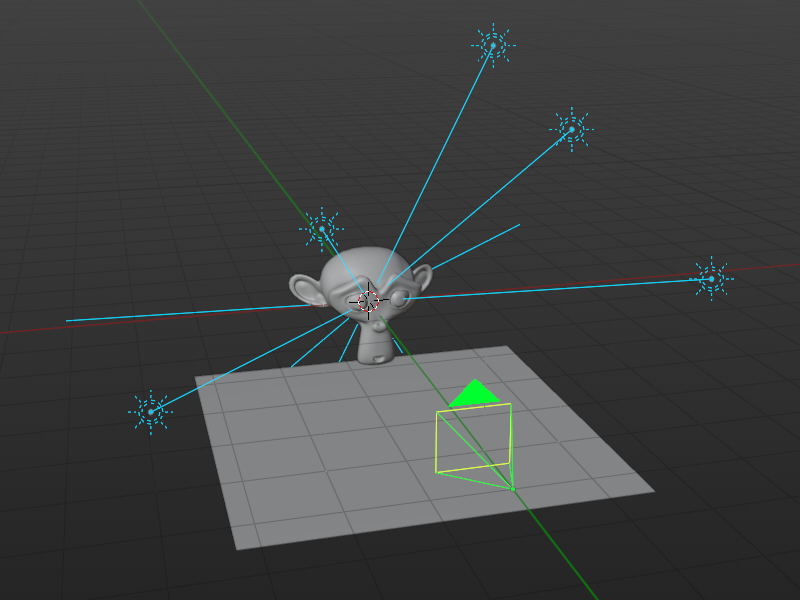
\includegraphics[width=0.5\columnwidth]{images/blender-scene_1.png}
  \nolinebreak
  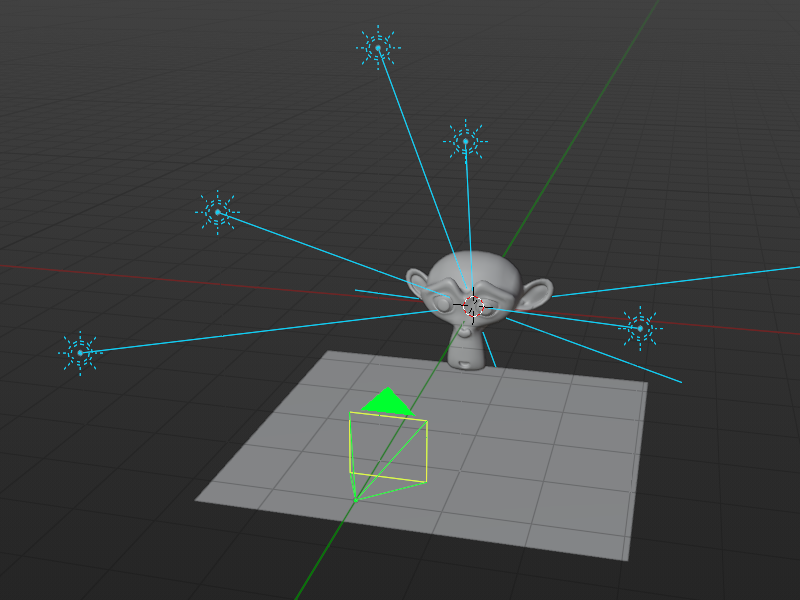
\includegraphics[width=0.5\columnwidth]{images/blender-scene_2.png}
  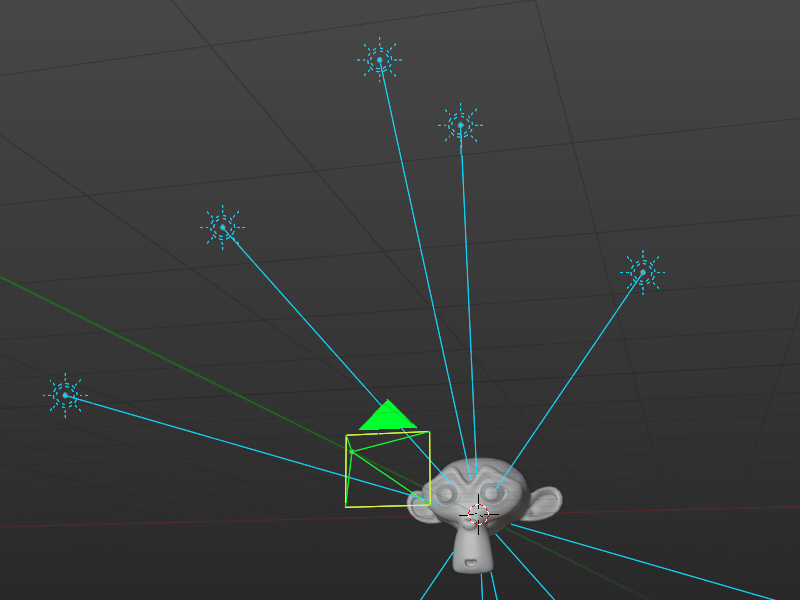
\includegraphics[width=0.5\columnwidth]{images/blender-scene_3.png}
  \nolinebreak
  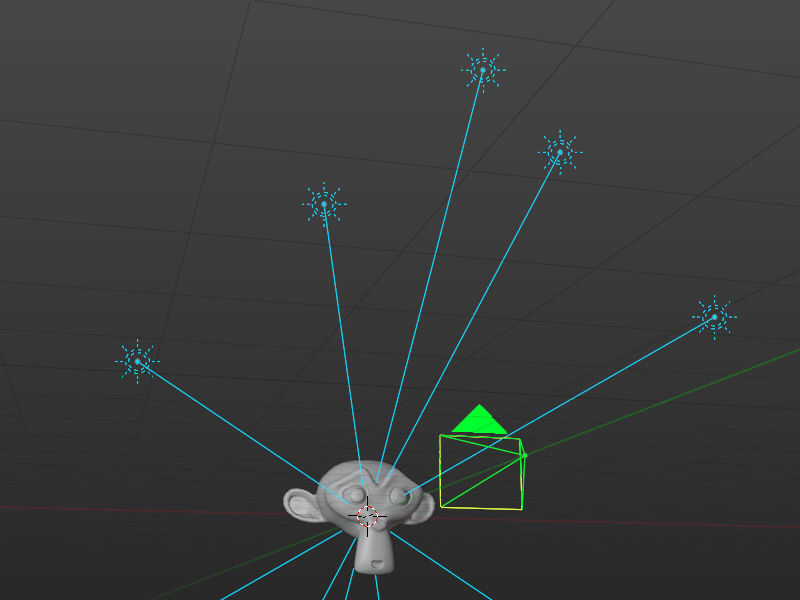
\includegraphics[width=0.5\columnwidth]{images/blender-scene_4.png}
  \caption{Four views of the scene in Blender used to render image data. Note
  that the positions of the light sources along their rays do not matter as
  they are purely directional.}\label{fig:blender-scene}
\end{figure}
\subsection{Least-Squares Approach}\label{sec:least-squares}
For each pixel location, we attempt to reconstruct the pixel according to
\begin{equation}
  \pixel_{i k} = \tilde{\light}_{i k} \point_k
\end{equation}
for each candidate $1 \le k \le 3^N$ and choose the one with the lowest squared
error
\begin{equation}
  \mathrm{error} = \sum_{i = 1}^N {\left(\pixel_i - \pixel_{i k}\right)}^2
\end{equation}
Note that this approach is only possible for $N \ge 4$. For $N = 3$, the
pseudoinverse in Equation~\ref{eq:pseudoinverse} is simply the inverse of
$\lights$ and the squared error is always zero.
\subsection{Forest-Building Approach}
By assumping the normal $\hat{\point} = \frac{\point}{\|\point\|}$ varies
smoothly across large regions of the object (its faces), we associate
candidates of $\point_k(x, y)$ with likely candidates $\point_k(x \pm 1, y)$
and $\point_k(x, y \pm 1)$ of its neighbors. We do using a variant on
breadth-first search: while processing $\point_k(x, y)$, we mark as its
neighbor the $\point_{k'}(x + 1, y)$ for
\begin{equation}
  \arg\max_{1 \le k' \le 3^N} \frac{\point_k(x, y) \cdot \point_{k'}(x + 1, y)}{\|\point_k(x, y)\| \, \|\point_{k'}(x + 1, y)\|}
\end{equation}
(the cosine similarity) and similarly with $\point_{k'}(x - 1, y)$,
$\point_{k'}(x, y + 1)$, and $\point_{k'}(x, y - 1)$. This forms a forest whose
connected components correspond to faces of the object. For a given pixel
position $(x, y)$, we take the candidate $\point$ that belongs to the largest
connected component.

This approach was only seriously considered due to an error in calculating its
complexity, which turns out to be $O \left({\left(3^n\right)}^3\right)$. As it
became clear that it was terribly impractical, this approach was abandoned.
\subsection{Energy-Minimizing Approach}
Instead of performing the costly forest construction described above, we could
pose the labelling task as an energy-minimization problem as described
in~\cite{schechner}. The objective function combines a data term to minimize
reconstruction error of $I_{i k}$ (as in Section~\ref{sec:least-squares}) as
well as a smoothness term that penalizes the difference in \emph{label} (that
is, the combination of sources visible to a pixel) rather than the difference
in the normal vector itself. Schechner et al.~\cite{schechner} propose a
graph-cut-based approximation to this otherwise NP-complete problem and
demonstrate that it is a reliable approach to light combination labelling for
photometric stereo with two or more lights per frame, which is exactly how we
characterize our mirrored problem.


  \section{Results}\label{sec:results}
Unfortunately, there turns out to be a fundamental contradiction that arises
when photometric stereo is attempted on a scene with a single stationary
perfect mirror: the total light vector when both the direct and reflected light
sources are visible to a pixel (the third case in
Equation~\ref{eq:combinations}) is \emph{always} coplanar, which is precisely
the situation in which Equation~\ref{eq:pseudoinverse} is underconstrained, due
to the pseudoinverse losing rank. As a result, none of the proposed approaches
would be capable of producing the correct normal vector, and a depth map could
not be recovered. See Figures~\ref{fig:output-candidates}
and~\ref{fig:output-combined} for a visualization of the output
of the least-squares approach.

To see why this is the case, consider the sum of $\light$ and $\light'$ in
Figure~\ref{fig:light-reflection}. Since $\light$ and $\light'$ always have the
same magnitude in the presense of a perfectly reflective mirror (one by which
light intensity is preserved), the vertical component cancels out and the
resulting vector is always parallel to the mirror plane. This is seen from
Equations~\ref{eq:light-reflection} and~\ref{eq:combinations}:
\begin{equation}
    \tilde{\light}_i = \light_i + \light_i'
                     = 2 \light_i - 2 \light_i^\parallel
                     = 2 \light_i^\perp
\end{equation}
Since the most common light combination is arguably this one in which neither
the direct nor the mirrored light is occluded, especially with shallow incident
light angles on the mirror surface, this is a significant handicap on the
utility of photometric stereo in the presence of such a mirror. Note that this
phenomenon only necessarily applies when the light is directional and the
mirror is stationary (i.e., its position does not vary between frames) and has
high reflectivity.
\begin{figure}
  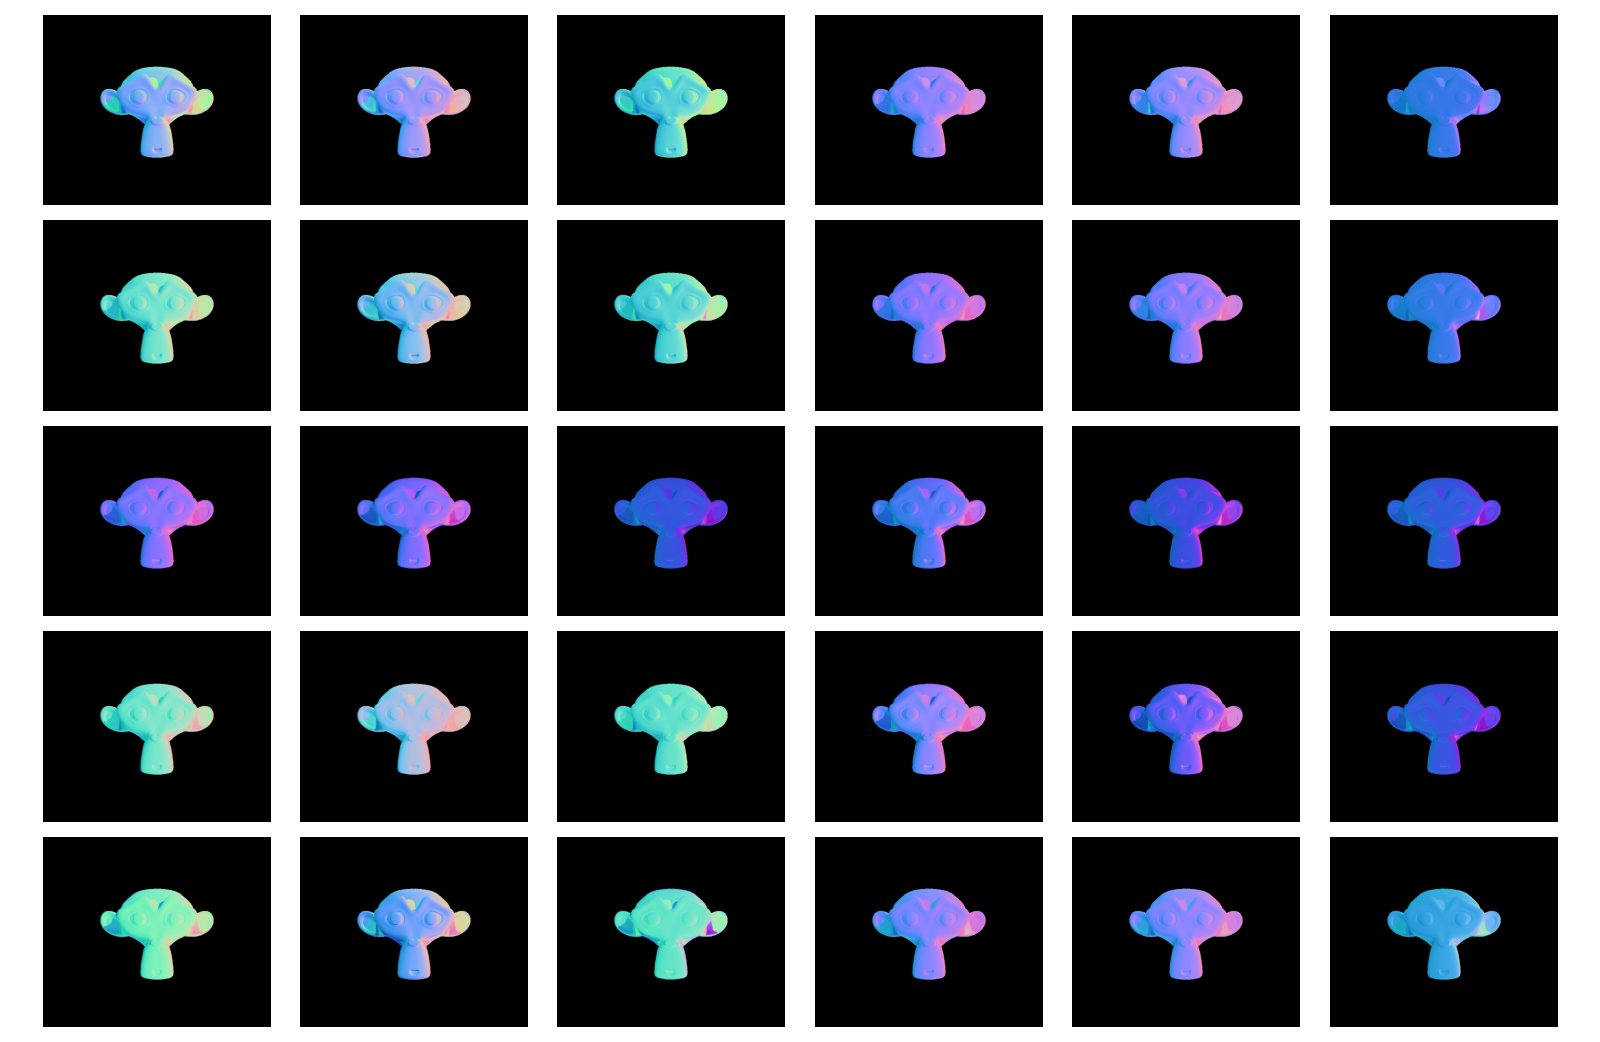
\includegraphics[width=\columnwidth]{images/output-candidates}
  \caption{A visualization of the first 30 of the 243 ($3^N$ with $N = 5$)
  computed normal maps assuming a different combination of light visible to the
  scene in each one. Within each of these candidate maps, the combination of
  lights incident on all pixels is assumed to be the same within a frame.
  Theoretically, the correct normal map can be constructed by selecting the
  correct option for each pixel among the candidates. Due to light source
  coplanarity and the subsequent loss of rank in the light matrix, the last
  such map (the one in which light from both the direct and the mirrored light
  sources is visible) is always blank.}\label{fig:output-candidates}
\end{figure}
\begin{figure}
  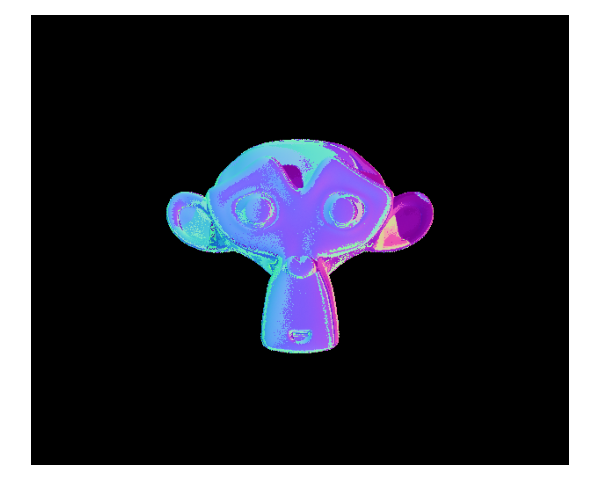
\includegraphics[width=\columnwidth]{images/output-combined}
  \caption{A visualization of the normal map constructed by the least-squares
  approach. Note that the most likely candidate for most pixels in the scene
  (the one in which all both the direct and the mirrored light sources is
  visible to a pixel in every frame) is invalid as described in
  Section~\ref{sec:results}. As a result, most of the obtained values are
  wrong.}\label{fig:output-combined}
\end{figure}


  \section{Conclusion}\label{sec:conclusion}
Photometric stereo is no doubt an essential component of the pantheon of
techniques for recovering 3D scene properties from purely visual information.
Making it work in difficult scenarios---scenes whose properties do not match
the original assumptions of light and surface properties---is an important
ongoing area of research.

In this paper, we looked at the applicability and implications of photometric
stereo in scenes containing a stationary perfect mirror, providing a
characterization of the problem and proposing a set of techniques for resolving
the inherent ambiguity that arises when multiple light sources---in this case,
the original light source and its mirror image---are present in a single frame.
Unfortunately, it appears that the basic linear problem of photometric stereo
is ill posed in the presence of such a mirror. We conclude with two statements:
that any setup for directional-light photometric stereo with mirrors requires
the mirrors to either change in position between frames or have a reflectivity
significantly less than 1, and that the task of photometric stereo with mirrors
in general reduces to a light-labelling problem of the sort described by
Schechner et al.\ in~\cite{schechner}, a problem for which the most efficient
solution still appears to be their ShadowCuts technique.
\subsection{Future Work}
Although the particular setup in our project was not condusive to a solution,
there are still plenty of questions worth pursuing in this space. The most
obvious is to continue investigating scenes for which photometric stereo
methods \emph{are} appropriate. As discussed above, these would be scenes in
which the mirror either changes in position from frame to frame or has a
reflectivity value of less than 1.

We might expect the former to have less utility due to its implications. If a
mirror is an inherent part of the scene, then it would not be likely (nor
desirable, as it implies scene motion) for the mirror to change position
between captures. If a mirror is part of the capture apparatus, then there
isn't a clear benefit of moving a mirror around between frames as opposed to
simply replacing it with another light source, which leads to a similar problem
characterization anyway. In fact, using a moving mirror instead of another
light souorce carries the additional drawback that a mirror can't simply be
switched on and off between frames as light sources are in~\cite{schechner}.

On the other hand, a mirror with lower reflectivity may be a simple solution to
this problem with no added complexity. The main drawback would be the lower
level of illumination on the object. It would be worth conducting further
experiments to see what values of reflectivity induce a good balance between
avoiding light vector coplanarity and providing enough illumination.

A second line of proposed future work involves modifying the characteristics of
the direct or reflected light in order to make it easier to pick apart the
direct and reflected illumination components on each pixel. Three approaches
are proposed:
\begin{enumerate}
  \item Apply a color filter to the mirror, so that it is only reflective for a
  subset of the incident wavelengths (from the direct illumination source).
  This can be combined with the lower-reflectivity mirror proposal above to
  reduce the number of custom components in the capture setup. A single mirror
  that reflects only red light with known non-unit reflectivity, for example,
  may work.
  \item Direct the incoming light at a glancing angle to the mirror surface.
  Because mirrors tend to induce polarization when reflecting light at shallow
  angles, the degree to which the light received by the sensor is polarized can
  be used to distinguish between direct and mirrored light sources.
  \item Use circularly polarized light in the direct source. Because mirrors
  reverse the direction of polarization, this can also be used as a way to
  distinguish between direct and mirrored light sources.
\end{enumerate}
Each of these three methods, by changing the characteristics of the mirrored
light with respect to the direct, may actually obviate the need for a
source-labelling algorithm as described in Section~\ref{sec:implementation}, as
the captured light would be more analogous to that of multi-band photometric
stereo, in which as few as a single image with multiple light channels can be
used to recover surface normals.


  {
    \small
    \bibliographystyle{ieee_fullname}
    \bibliography{references}
  }
  \newpage
  \section*{A. Assets}
All code and data used can be found at
\url{https://github.com/deeptoaster/16-823-project} (with the exception of the
DiLiGenT dataset, which is available from~\cite{shi}).
\section*{B. Art}
Although the output as shown in Section~\ref{sec:results} was not quite what
was desired, I did find some of the accidental images produced throughout the
process amusing. Here are some highlights.
\begin{figure}[h]
  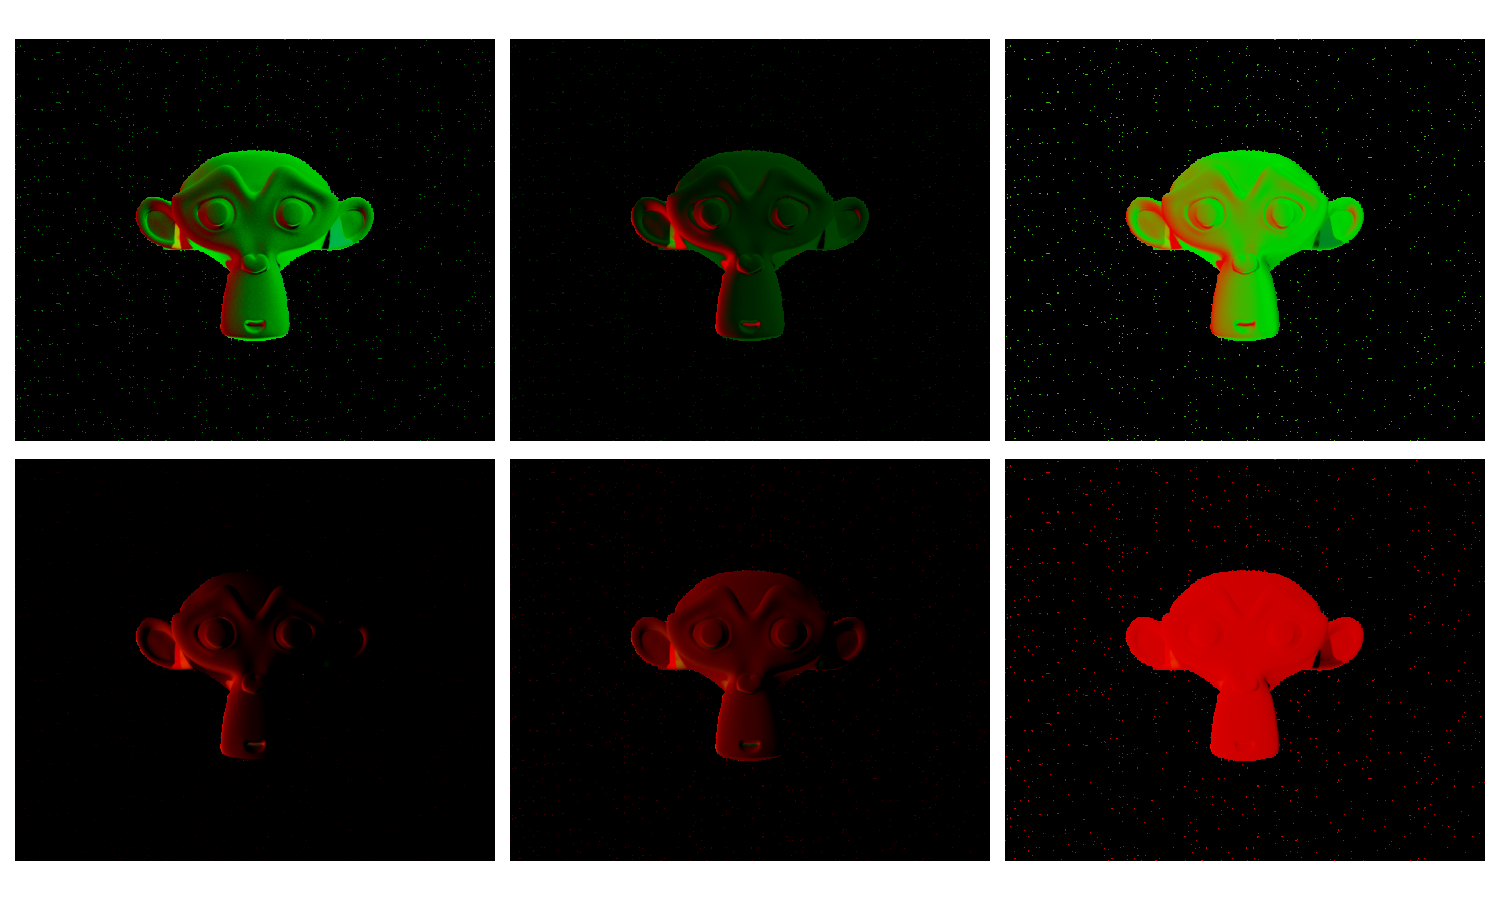
\includegraphics[width=\columnwidth]{images/space-monkey-mafia}
  \caption{Space Monkey Mafia (2023).}
\end{figure}
\begin{figure}[h]
  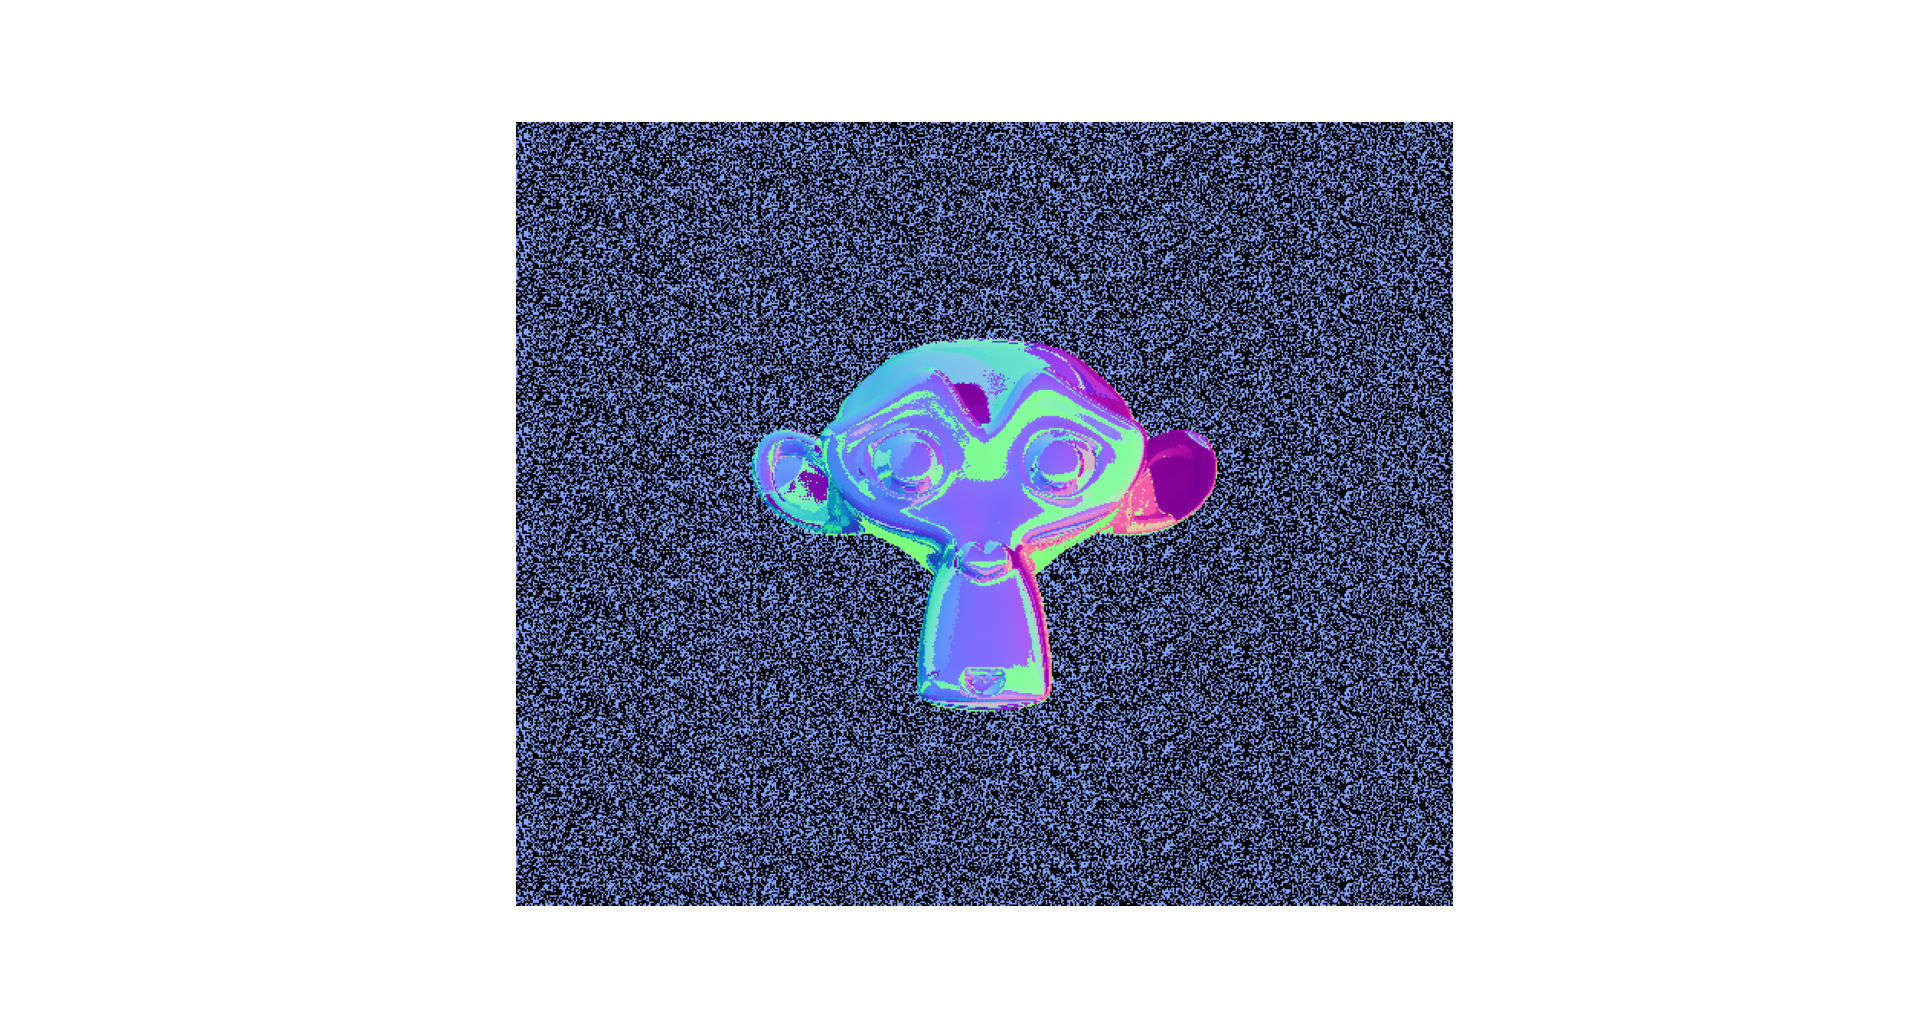
\includegraphics[width=\columnwidth]{images/vaporwave}
  \caption{Vaporwave (2023).}
\end{figure}


\end{document}

